\documentclass[10pt,a4paper]{report}
\usepackage[utf8]{inputenc}
\usepackage[francais]{babel}
\usepackage[T1]{fontenc}
\usepackage{amsmath}
\usepackage{amsfonts}
\usepackage{amssymb}

\usepackage{algorithm}
\usepackage{algpseudocode}

\usepackage{hyperref}

\usepackage{graphicx}
\usepackage{fancyvrb}

\renewcommand{\thesection}{\arabic{section}}
\newcommand{\HRule}{\rule{\linewidth}{0.5mm}}
\VerbatimFootnotes


\begin{document}

\begin{titlepage}
\begin{center}

%\def\authors#1{\def\@authors{#1}}
%\newcommand{\printauthors}{\@authors}

% Upper part of the page. The '~' is needed because \\
% only works if a paragraph has started.
%\includegraphics[width=0.75\textwidth]{images/FileHub}~\\[2cm]

% \textsc{\LARGE UFR Sciences d'Angers}\\[1.5cm]

% \textsc{\huge FileHub}\\[1cm]

% Title
\HRule \\[0.4cm]
{ \huge \bfseries probleme des n dames \\[0.4cm] }

\HRule \\[1.5cm]

% Author and supervisor
\begin{minipage}{0.4\textwidth}
\begin{flushleft} \large
\emph{Auteurs:}\\
\textsc{Frémont} Alexandre\\
\textsc{Le Calvar} Théo\\

\end{flushleft}
\end{minipage}
\begin{minipage}{0.4\textwidth}
\begin{flushright} \large
\emph{Référent:} \\
\textsc{Lesaint} David \\
\textsc{Hao} Jin-Kao 
\end{flushright}
\end{minipage}

\vfill

% Bottom of the page
{\large Février 2015}

\end{center}
\end{titlepage}

\tableofcontents

\newpage

% \section{Résumé du projet}
\section{Résumé du projet}

Le problème des N-Dames est une extension du problème des 8 dames, son but est de placer 8 dames d'un jeu d'échecs sur un échiquier de façon à ce qu'aucune ne soit menacée.
Pour notre problème, nous ne considérons non plus un échiquier de $8*8$ cases, mais sur un échiquier arbitrairement grand. On peut démontrer que pour tout $n >= 4$ il existe au moins une solution.

Dans ce rapport nous présenterons les algorithmes et les structures mis en place pour résoudre l'approche programmation par contrainte de ce problème.

Ce projet a été développé en C, car ce langage nous permettait un contrôle fin de la mémoire, point particulièrement important.
À cause du fait que nous voulions avoir un programme proposant des algorithmes de résolutions utilisant la programmation par contrainte et la recherche locale nous avons dû mettre en place une structure de données commune.
Nous avons mis en place deux algorithmes, le backtracking et le forward checking.

Tous les tests de performance ont été effectués sur un Intel(R) Core(TM) i7-2600K CPU @ 4.20GHz accompagné de 16Go de RAM cadencée à 1.600 MHz.


% \section{structure de données}
\section{Structure de données}

Pour représenter un échiquier, nous avons décidé d'utiliser un tableau à une dimension où chaque case représente l'emplacement d'une dame.
Ainsi l'indice du tableau correspond à la colonne de l'échiquier et la valeur à la ligne.
Il est possible d'intervertir la signification des indices et des valeurs, les deux solutions représentent deux échiquiers symétriques par la diagonale.
Cette représentation présente l'immense avantage d'éliminer par construction les conflits sur les lignes et les colonnes (si l’on fait attention à ne pas introduire deux fois la même valeur dans le tableau),
limitant donc les conflits aux diagonales.

De plus, parce que chaque méthode de résolution nécessitait des informations complémentaires (gestion des domaines de valeurs pour le forward checking, maintient des conflits pour la recherche locale),
nous avons choisi de réduire la structure d'échiquier à son strict minimum et que chaque méthode apporterait ses structures complémentaires.

Ainsi le forward checking utilise un tableau de bitsets pour représenter les domaines, le backtracking lui, tient juste à jour un bitset contenant les lignes disponibles.


% \section{backtrack}
\section{Backtracking}

Le backtracking est un algorithme récursif générique. Son principe est de parcourir l'espace de recherche grâce à un arbre.
Cet algorithme présente l'avantage d'être simple à mettre en place sur des problèmes comme celui des N-Dames ou la résolution de grille de sudoku, cependant comme nous le verrons, il a l'inconvénient d'être assez peu performant.

L'idée globale est de tester toutes les branches de l'arbre, mais de s'arrêter dès qu'un noeud mène à une instanciation partielle qui ne peut être valide (dames en conflits pour notre problème).
Grâce à cela, de nombreuses configurations ne sont pas testées, ce qui réduit l'espace de recherche.

Notre implémentation diffère d'un backtracking naïf, car lors de la génération du noeud nous limitons les valeurs possibles de la nouvelle dame aux cases qui ne seront pas en conflit avec les dames posées précédemment.

Grâce à cela nous obtenons des résultats corrects.

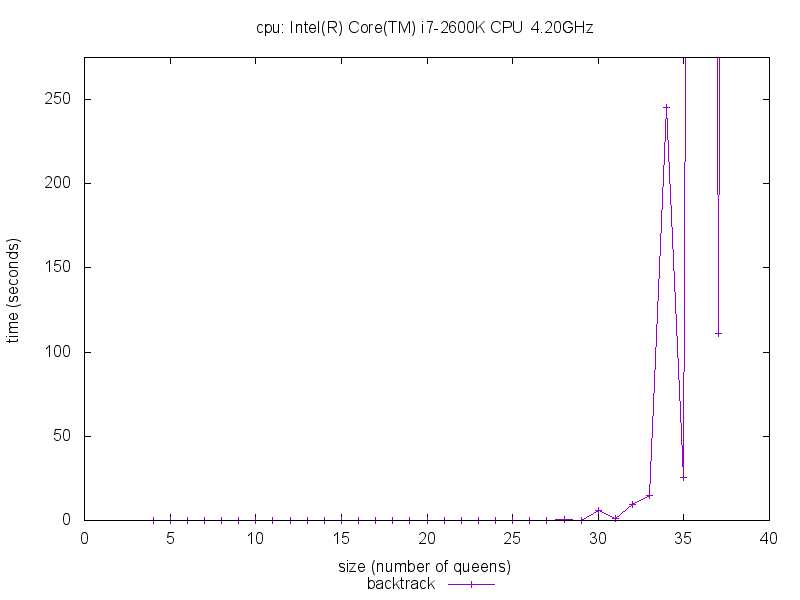
\includegraphics[width=1\textwidth]{images/plot_bt_i7.png}

Notre algorithme résout les échiquiers de tailles $n <= 28$ en moins d'une seconde. Après on remarque la brusque augmentation du temps due à l'explosion de la taille de l'espace de recherche.
On remarque aussi un schéma, les tailles impaires sont globalement bien plus rapides à calculer que les tailles paires. En effet, sur les tailles paires la première solution est assez éloignée de la configuration en cavalier.
Ceci n'est pas visible sur le graphique, mais on remarque aussi certaines tailles pour lesquelles l’exécution est particulièrement longue ($36$ et $40$).
On pourra se reporter à ce \url{http://queens.cspea.co.uk/csp-q-allplaced.html} qui liste le nombre de solutions testées avant de trouver la première configuration valide.

Après réflexion il nous semblait peu pertinent d'implémenter les algorithmes d'Arc Consistency, en effet, ceux-ci sont sont contre performant dans le cas du problème des N-Dames, les contraintes du problème sont des
\textit{tous differents} or ce type de contrainte ne réduit que très peu les domaines restants (voir pas du tout dans le cas d'une exécution précédant la recherche de solution).
Nous avons donc préféré nous attarder sur le forward checking qui lui présente un intérêt pour ce problème.

\break
% \section{forward checking}
\section{Forward checking}

Le forward checking, comme le backtracking, est une solution générique. Il reprend l'idée de parcourir l'espace de recherche du problème grâce à un arbre.
Cependant, à chaque variable (ici dame) est associé son domaine (les cases de sa colonne où elle peut être placée).
À chaque placement d'une nouvelle dame, on retire des domaines des dames non placées les valeurs qui rentrent en conflit avec la dame placée.
Si un domaine vient à ne plus contenir aucune valeur alors forcément il n'existe pas de solutions pour cette branche et il faut revenir sur des placements précédents.
Cette technique réduit encore l'espace de recherche comparé au backtracking.

Dans notre implémentation nous avons choisi d'utiliser un tableau de bitset pour représenter les domaines.
Un bit indique donc si la dame peut être placée à cette position.
Pour ne pas avoir à recalculer les domaines à chaque noeud nous avons décidé de conserver un unique tableau de domaines qui sera modifié lors de chaque appel récursif.
Nous avons donc dû trouver une solution pour conserver les différences appliquées par chaque noeud aux domaines pour pouvoir les défaire en cas de backtrack.
Ainsi pour chaque noeud nous tenons à jour un tableau $delta$ où sont stockées 3 informations par colonne du tableau,
s'il faut remettre à 1 le bit de la ligne, de la diagonale montante ou de la diagonale descendante lors du nettoyage des domaines.
Le choix de la prochaine dame à placer se fait par l'heuristique du plus petit domaine.

Grâce à tout cela, nous obtenons des résultats corrects, bien que limités.

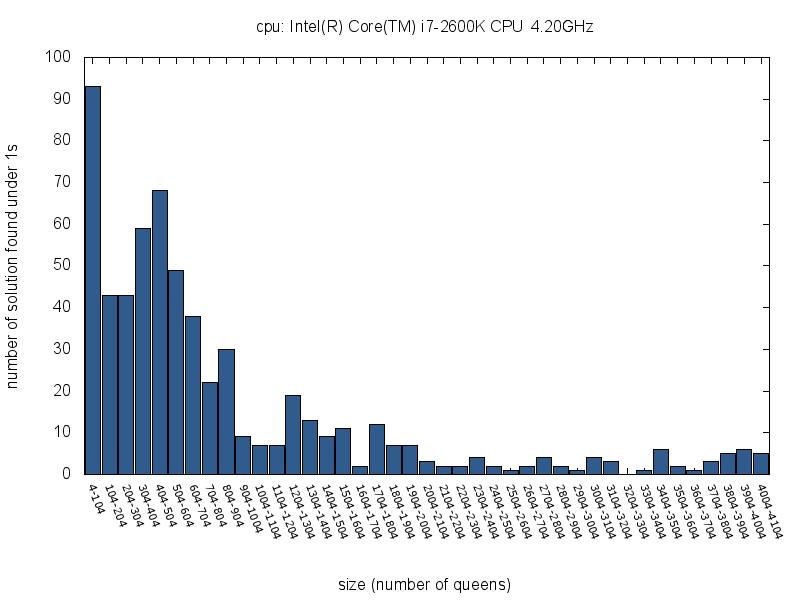
\includegraphics[width=1\textwidth]{images/plot_fw_i7.png}

Le graphique représente le nombre de solutions trouvées en moins d'une seconde par tranche de 100.
Lors de l'exécution, nous avons remarqué des valeurs pour lesquelles l'algorithme était particulièrement lent (visibles sur le prochain graphique).
Nous avons choisi de tester notre algorithme jusqu'au maximum autorisé par nos structures de données (pour des $n >= 1024$ il est nécessaire d'augmenter la limite de stack) par curiosité plus que réel intérêt.
En effet, on remarque que passé les 600 le nombre de solutions trouvées rapidement est vraiment bas (moins de 50\%) et que notre algorithme n'est plus adapté.
Il est possible de chercher plus longtemps pour obtenir quelques solutions supplémentaires. La quasi-totalité des solutions inférieures à 200 se trouve en moins de 5 minutes.


Voici un graphique comparant les temps d'exécution pour les tailles allant de 4 à 100.

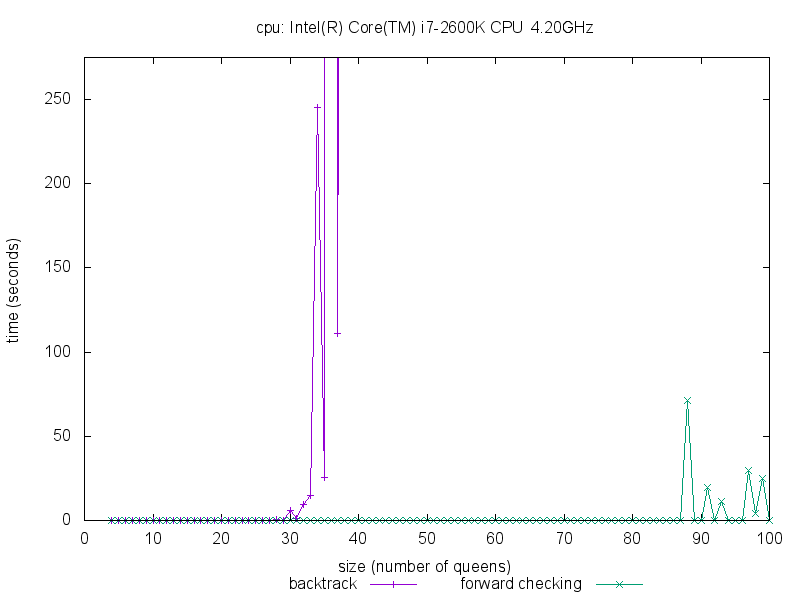
\includegraphics[width=0.8\textwidth]{images/plot_bt_fw_i7.png}

Le constat est sans appel, le forward checking est bien plus performant que le backtrack. Il permet de calculer en moins d'une seconde des tailles qui avec le backtracking seraient calculées en semaines voir en mois.

\section{Conclusion}

Les algorithmes de backtracking et de forward checking sont des méthodes déterministes. En effet, ils assurent la découverte d'une solution si elle existe.
Cependant ils n'assurent pas une exécution dans un temps raisonnable\footnote{On peut penser à la réponse à la grande question sur la vie, l'univers et le reste que \textit{Deep Thought} calcule pendant 7.5 millions d'années.}.
Ce problème est particulièrement visible sur l'algorithme de backtracking, malgré des valeurs relativement petites le temps d'exécution s'envole.
L'algorithme de forward checking repousse un peu la limite, mais ne résout pas le problème.
En effet, le seul moyen efficace de trouver des solutions de grandes tailles à ces problèmes est d'utiliser une recherche locale ou un autre algorithme qui ne cherchera pas à parcourir l'espace de recherche de manière systématique.
Nous avons réussi à implémenter une recherche locale trouvant en environ 13 minutes une solution de taille $1,000,000,000$ alors qu'il faut plus de 30 minutes pour trouver une solution de taille 36 avec l'algorithme de backtrack.



\end{document}
